%compile with XeLaTeX
\documentclass[9pt,a4paper,oneside]{report}
\usepackage[margin=18mm,landscape]{geometry}
\usepackage{xltxtra,fontspec,xunicode} %requires XeLaTeX
  \setromanfont{Source Sans Pro}
  \setsansfont{Source Sans Pro}
  \setmonofont{DejaVu Sans Mono}
\usepackage{fancyhdr}
\pagestyle{fancy}
\chead{\url{http://reqT.org/reqT-cheat-sheet.pdf}}
\usepackage{hyperref}
\hypersetup{colorlinks=true, linkcolor=blue, urlcolor=blue}
\usepackage[usenames,dvipsnames,svgnames,table]{xcolor}
\definecolor{entityColor}{RGB}{0,100,200}
\definecolor{attributeColor}{RGB}{0,100,50}
\definecolor{relationColor}{RGB}{160,0,30}
\usepackage{listings}
\lstdefinestyle{reqT}{
  %belowcaptionskip=1\baselineskip,
  breaklines=true,
  %showstringspaces=false,
  showspaces=false,
  %breakatwhitespace=true,
  basicstyle=\ttfamily\small,
  emph={Ent,Meta,Item,Label,Section,Term,Actor,App,Component,Domain,Module,Product,Release,Resource,Risk,Service,Stakeholder,System,User,Class,Data,Input,Member,Output,Relationship,Design,Screen,MockUp,Function,Interface,State,Event,Epic,Feature,Goal,Idea,Issue,Req,Ticket,WorkPackage,Breakpoint,Barrier,Quality,Target,Scenario,Task,Test,Story,UseCase,VariationPoint,Variant},
  emphstyle=\bfseries\color{entityColor},
  emph={[2]has,is,superOf,binds,deprecates,excludes,helps,hurts,impacts,implements,interactsWith,precedes,requires,relatesTo,verifies},
  emphstyle={[2]\bfseries\color{relationColor}},
  emph={[3]Attr,Code,Constraints,Comment,Deprecated,Example,Expectation,FileName,Gist,Image,Spec,Text,Title,Why,Benefit,Capacity,Cost,Damage,Frequency,Min,Max,Order,Prio,Probability,Profit,Value,Status},
  emphstyle={[3]\bfseries\color{attributeColor}},  
}
\lstset{style=reqT}
\usepackage{multicol}

\setlength\parindent{0em}
\usepackage{titlesec}
  \titlespacing{\section}{0pt}{5pt}{2pt}
  \titlespacing{\subsection}{0pt}{5pt}{2pt}
  \titlespacing{\subsubsection}{0pt}{5pt}{2pt}
  
\usepackage{graphicx}
%\frenchspacing
\begin{document}
\begin{multicols*}{4}
    \section*{Entity}

\subsection*{General}

\hangindent=1em\lstinline+Item+  An article in a collection, enumeration, or series.

\hangindent=1em\lstinline+Label+ A descriptive name used to identify something.

\hangindent=1em\lstinline+Meta+ A prefix used on a concept to mean beyond or about its own concept, e.g. metadata is data about data.

\hangindent=1em\lstinline+Section+ A part of a (requirements) document.

\hangindent=1em\lstinline+Term+ A word or group of words having a particular meaning.

\subsection*{Context}

\hangindent=1em\lstinline+Actor+ A human or machine that communicates with a system.

\hangindent=1em\lstinline+App+ A computer program, or group of programs designed for end users, normally with a graphical user interface. Short for application.

\hangindent=1em\lstinline+Component+ A composable part of a system. A reusable, interchangeable system unit or functionality.

\hangindent=1em\lstinline+Domain+ An application area. A product and its surrounding entities.

\hangindent=1em\lstinline+Module+ A collection of coherent functions and interfaces.

\hangindent=1em\lstinline+Product+ Something offered to a market.

\hangindent=1em\lstinline+Release+ A specific version of a system offered at a specific time to end users.

\hangindent=1em\lstinline+Resource+ A capability of, or support for development.

\hangindent=1em\lstinline+Risk+ Something negative that may happen.

\hangindent=1em\lstinline+Service+ Actions performed by systems and/or humans to provide results to stakeholders.

\hangindent=1em\lstinline+Stakeholder+ Someone with a stake in the system development or usage.

\hangindent=1em\lstinline+System+ A set of interacting software and/or hardware components.

\hangindent=1em\lstinline+User+ A human interacting with a system.

\subsection*{Requirement}

\subsubsection*{DataReq}

\hangindent=1em\lstinline+Class+ An extensible template for creating objects. A set of objects with certain attributes in common. A category.

\hangindent=1em\lstinline+Data+ Information stored in a system.

\hangindent=1em\lstinline+Input+ Data consumed by an entity, 

\hangindent=1em\lstinline+Member+ An entity that is part of another entity, eg. a field in a in a class.

\hangindent=1em\lstinline+Output+ Data produced by an entity, e.g. a function or a test.

\hangindent=1em\lstinline+Relationship+ A specific way that entities are connected.

\subsubsection*{DesignReq}

\hangindent=1em\lstinline+Design+ A specific realization or high-level implementation description (of a system part).

\hangindent=1em\lstinline+Screen+ A design of (a part of) a user interface.

\hangindent=1em\lstinline+MockUp+ A prototype with limited functionality used to demonstrate a design idea.

\subsubsection*{FunctionalReq}

\hangindent=1em\lstinline+Function+ A description of how input data is mapped to output data. A capability of a system to do something specific.

\hangindent=1em\lstinline+Interface+ A defined way to interact with a system.

\hangindent=1em\lstinline+State+ A mode or condition of something in the domain and/or in the system. A configuration of data.

\hangindent=1em\lstinline+Event+ Something that can happen in the domain and/or in the system.

\subsubsection*{GeneralReq}

\hangindent=1em\lstinline+Epic+ A large user story or a collection of stories.

\hangindent=1em\lstinline+Feature+ A releasable characteristic of a product. A (high-level, coherent) bundle of requirements.

\hangindent=1em\lstinline+Goal+ An intention of a stakeholder or desired system property.

\hangindent=1em\lstinline+Idea+ A concept or thought (potentially interesting).

\hangindent=1em\lstinline+Issue+ Something needed to be fixed.

\hangindent=1em\lstinline+Req+ Something needed or wanted. An abstract term denoting any type of information relevant to the (specification of) intentions behind system development. Short for requirement.

\hangindent=1em\lstinline+Ticket+ (Development) work awaiting to be completed.

\hangindent=1em\lstinline+WorkPackage+ A collection of (development) work tasks.

\subsubsection*{QualityReq}

\hangindent=1em\lstinline+Breakpoint+ A point of change. An important aspect of a (non-linear) relation between quality and benefit.

\hangindent=1em\lstinline+Barrier+ Something that makes it difficult to achieve a goal or a higher quality level.

\hangindent=1em\lstinline+Quality+ A distinguishing characteristic or degree of goodness.

\hangindent=1em\lstinline+Target+ A desired quality level or goal .

\subsubsection*{ScenarioReq}

\hangindent=1em\lstinline+Scenario+ A (vivid) description of a (possible future) system usage.

\hangindent=1em\lstinline+Task+ A piece of work (that users do, maybe supported by a system).

\hangindent=1em\lstinline+Test+ A procedure to check if requirements are met.

\hangindent=1em\lstinline+Story+ A short description of what a user does or needs. Short for user story.

\hangindent=1em\lstinline+UseCase+ A list of steps defining interactions between actors and a system to achieve a goal.

\subsubsection*{VariabilityReq}

\hangindent=1em\lstinline+VariationPoint+ An opportunity of choice among variants.

\hangindent=1em\lstinline+Variant+ An object or system property that can be chosen from a set of options.

\section*{RelationType}

\hangindent=1em\lstinline+binds+ Ties a value to an option. A configuration binds a variation point.

\hangindent=1em\lstinline+deprecates+ Makes outdated. An entity deprecates (supersedes) another entity.

\hangindent=1em\lstinline+excludes+ Prevents a combination. An entity excludes another entity.

\hangindent=1em\lstinline+has+ Expresses containment, substructure. An entity contains another entity.

\hangindent=1em\lstinline+helps+ Positive influence. A goal helps to fulfil another goal.

\hangindent=1em\lstinline+hurts+ Negative influence. A goal hinders another goal.

\hangindent=1em\lstinline+impacts+ Some influence. A new feature impacts an existing component.

\hangindent=1em\lstinline+implements+ Realisation of. A module implements a feature.

\hangindent=1em\lstinline+interactsWith+ Communication. A user interacts with an interface.

\hangindent=1em\lstinline+is+ Sub-typing, specialization, part of another, more general entity.

\hangindent=1em\lstinline+precedes+ Temporal ordering. A feature precedes (is implemented before) another feature.

\hangindent=1em\lstinline+requires+ Requested combination. An entity is required (or wished) by another entity.

\hangindent=1em\lstinline+relatesTo+ General relation. An entity is related to another entity.

\hangindent=1em\lstinline+superOf+ Super-typing, generalization, includes another, more specific entity.

\hangindent=1em\lstinline+verifies+ Gives evidence of correctness. A test verifies the implementation of a feature.

\section*{Attribute}

\subsection*{StringAttribute}

\hangindent=1em\lstinline+Code+ A collection of (textual) computer instructions in some programming language, e.g. Scala. Short for source code.

\hangindent=1em\lstinline+Comment+ A note that explains or discusses some entity.

\hangindent=1em\lstinline+Deprecated+ A description of why an entity should be avoided, often because it is superseded by another entity, as indicated by a 'deprecates' relation.

\hangindent=1em\lstinline+Example+ A note that illustrates some entity by a  typical instance.

\hangindent=1em\lstinline+Expectation+ The required output of a test in order to be counted as passed.

\hangindent=1em\lstinline+FileName+ The name of a storage of serialized, persistent data.

\hangindent=1em\lstinline+Gist+ A short and simple description of an entity, e.g. a function or a test.

\hangindent=1em\lstinline+Image+ (The name of) a picture of an entity.

\hangindent=1em\lstinline+Spec+ A (detailed) definition of an entity. Short for specification

\hangindent=1em\lstinline+Text+ A sequence of words (in natural language).

\hangindent=1em\lstinline+Title+ A general or descriptive heading.

\hangindent=1em\lstinline+Why+ A description of intention. Rationale.

\subsection*{IntAttribute}

\hangindent=1em\lstinline+Benefit+ A characterisation of a good or helpful result or effect (e.g. of a feature).

\hangindent=1em\lstinline+Capacity+ The largest amount that can be held or contained (e.g. by a resource).

\hangindent=1em\lstinline+Cost+ The expenditure of something, such as time or effort, necessary for the implementation of an entity.

\hangindent=1em\lstinline+Damage+ A characterisation of the negative consequences if some entity (e.g. a risk) occurs.

\hangindent=1em\lstinline+Frequency+ The rate of occurrence of some entity. 

\hangindent=1em\lstinline+Min+ The minimum estimated or assigned (relative) value.

\hangindent=1em\lstinline+Max+ The maximum estimated or assigned (relative) value.

\hangindent=1em\lstinline+Order+ The ordinal number of an entity (1st, 2nd, ...).

\hangindent=1em\lstinline+Prio+ The level of importance of an entity. Short for priority.

\hangindent=1em\lstinline+Probability+ The likelihood that something (e.g. a risk) occurs.

\hangindent=1em\lstinline+Profit+ The gain or return of some entity, e.g. in monetary terms.

\hangindent=1em\lstinline+Value+ An amount. An estimate of worth.

\subsection*{StatusValueAttribute}

\hangindent=1em\lstinline+Status+ A level of refinement of an entity (e.g. a feature) in the development process. 

\subsection*{VectorAttribute}

\hangindent=1em\lstinline+Constraints+ A collection of propositions that restrict the possible values of a set of variables.

\vspace{2em}
\section*{Tree-like Model Structure}

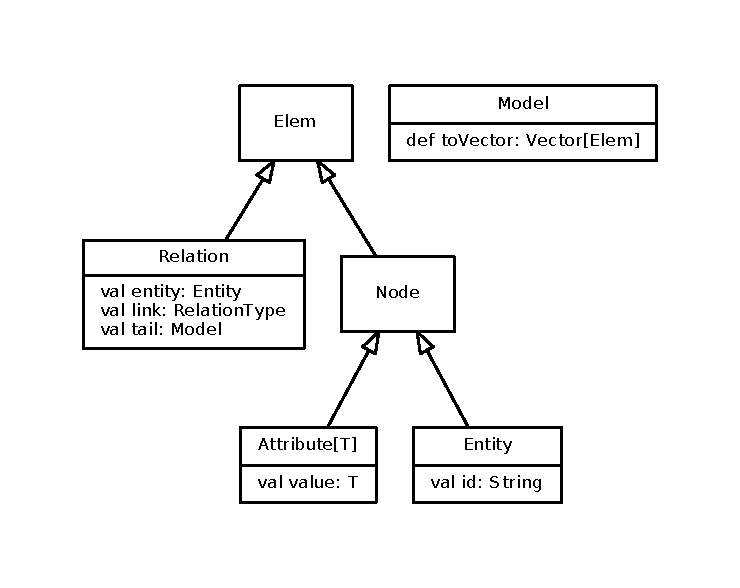
\includegraphics[width=6.3cm]{metamodel.pdf}

\vspace{2em}
\section*{Model Scripting}
\subsection*{Model Construction}
A Model has a body within parentheses with a comma-separated sequence of zero or more Elems. A relation links an Entity with a submodel body including a sequence of zero or more Elems.
\begin{lstlisting}
var m = Model(  
  Title("example"), 
  Feature("helloWorld") has 
    Spec("Print hello msg."),
  Stakeholder("x") requires (
    Req("nice") has (
      Prio(10),
      Gist("gimme this")),
    Req("cool") has (
      Prio(5),
      Gist("better have it")
    )
  )
)   
\end{lstlisting}

\subsection*{Model Operations}

Add element to a Model m: 
\begin{lstlisting}
m + (Req("r") has Prio(42))
\end{lstlisting}

Remove elements from a Model m:
\begin{lstlisting}
m - Req("nice") - Title
\end{lstlisting}

Collecting Int values in a Vector[Int]:
\begin{lstlisting}
m.collect{case Prio(i) => i}
\end{lstlisting}

Collecting entities in a new Model:
\begin{lstlisting}
m.collect{case r: Req => r}.toModel
\end{lstlisting}

Transforming Entity type in a new Model:
\begin{lstlisting}
m.transform{
  case Req(id) => Feature(id)
}
\end{lstlisting}

\subsection*{Release Constraint Solving}
\begin{lstlisting}[basicstyle=\ttfamily\scriptsize]
val simplePlan = Model(
  Stakeholder("X") has (
    Prio(1),
    Feature("1") has Benefit(4),
    Feature("2") has Benefit(2),
    Feature("3") has Benefit(1)),
  Stakeholder("Y") has (
    Prio(2),
    Feature("1") has Benefit(2),
    Feature("2") has Benefit(1),
    Feature("3") has Benefit(1)),
  Release("A") precedes Release("B"),  
  Resource("dev") has (
    Feature("1") has Cost(10),
    Feature("2") has Cost(70),
    Feature("3") has Cost(40),
    Release("A") has Capacity(100),
    Release("B") has Capacity(100)),
  Resource("test") has (
    Feature("1") has Cost(40),
    Feature("2") has Cost(10),
    Feature("3") has Cost(70),
    Release("A") has Capacity(100),
    Release("B") has Capacity(100)),
  Feature("3") precedes Feature("1"))
val problem = csp.releasePlan(simplePlan)
val solution = 
  problem.maximize(Release("A")/Benefit)
val sortedSolution = 
  solution.sortByTypes(Release, Feature, Stakeholder, Resource)
\end{lstlisting}

\subsection*{Model Export}
\begin{lstlisting}
reqT.export.toGraphVizNested(m).
  save("filename.dot")
\end{lstlisting}
Available exporters:
\begin{lstlisting}
toGraphVizNested  
toGraphVizFlat  
toPathTable
toHtml
toText
toLatex
toQuperSpec
\end{lstlisting}
\end{multicols*}

\end{document}